\documentclass[table]{beamer}
\mode<presentation>
\usetheme{Berlin}
\usecolortheme{beaver}
\usepackage{listings}
\usepackage{multirow}
\usepackage{xcolor}

%%%
% LISTINGS SETTING
\lstset{ %
  backgroundcolor=\color{yellow},   % choose the background color; you must add \usepackage{color} or \usepackage{xcolor}
  basicstyle=\tiny\ttfamily,        % the size of the fonts that are used for the code
  breakatwhitespace=false,         % sets if automatic breaks should only happen at whitespace
  breaklines=true,                 % sets automatic line breaking
  captionpos=b,                    % sets the caption-position to bottom
  commentstyle=\color{red},    % comment style
  deletekeywords={...},            % if you want to delete keywords from the given language
  escapeinside={\%*}{*)},          % if you want to add LaTeX within your code
  extendedchars=true,              % lets you use non-ASCII characters; for 8-bits encodings only, does not work with UTF-8
  frame=single,                    % adds a frame around the code
  keepspaces=true,                 % keeps spaces in text, useful for keeping indentation of code (possibly needs columns=flexible)
  keywordstyle=\color{blue},       % keyword style
%  language=Octave,                 % the language of the code
  morekeywords={*,...},            % if you want to add more keywords to the set
  numbers=left,                    % where to put the line-numbers; possible values are (none, left, right)
  numbersep=5pt,                   % how far the line-numbers are from the code
  numberstyle=\tiny\color{gray}, % the style that is used for the line-numbers
  rulecolor=\color{black},         % if not set, the frame-color may be changed on line-breaks within not-black text (e.g. comments (green here))
  showspaces=false,                % show spaces everywhere adding particular underscores; it overrides 'showstringspaces'
  showstringspaces=false,          % underline spaces within strings only
  showtabs=false,                  % show tabs within strings adding particular underscores
  stepnumber=1,                    % the step between two line-numbers. If it's 1, each line will be numbered
  stringstyle=\color{violet},     % string literal style
  tabsize=4,                       % sets default tabsize to 2 spaces
  title=\lstname                   % show the filename of files included with \lstinputlisting; also try caption instead of title
}

%%%
% TITLE PREAMBLE
\title[Intro to Bioinformatics] % (optional, only for long titles)
{An Introduction to Bioinformatics Tools}
\subtitle{Part 1: Golden Rules of Bioinformatics}
\author[Pritchard, Cock] % (optional, for multiple authors)
{Leighton~Pritchard \and Peter~Cock}
\institute[The James Hutton Institute] % (optional)
{
  Information and Computational Sciences\\
  The James Hutton Institute
}
\date[May 2014] % (optional)
{Bioinformatics Training, 29$^{th}$, 30$^{th}$ May 2014}
\subject{Bioinformatics}

%%%
% TOC
% Show table of contents, with current section highlighted,
% at the start of each section
\AtBeginSection[]
{
  \begin{frame}
    \frametitle{Table of Contents}
    \tableofcontents[currentsection]
  \end{frame}
}


%%%
% START DOCUMENT
\begin{document}

  \frame[plain]{\titlepage}
  
  \begin{frame}
    \frametitle{Bertrand Russell}
    \begin{center}
      
\includegraphics[width=\textwidth]{images/bertrand}
    \end{center}
  \end{frame}
    
 %%%
 % SECTION: The Golden Rules of Bioinformatics
  \section{The Golden Rules of Bioinformatics}

  \subsection{Rule 0}
  \begin{frame}
    \frametitle{Zeroeth Golden Rule of Bioinformatics}
    \framesubtitle{Always communicate}
	\begin{itemize}
	  \item No-one knows everything about everything - talk to people!
	  \begin{itemize}
	    \item local bioinformaticians, mailing lists, forums, Twitter, etc.
	  \end{itemize}
	  \item Keep learning - there are lots of resources
	  \item There is no free lunch - no method works best on all data
	  \item The worst errors are silent - share worries, problems, etc.
	  \item Share expertise (see first item)
	\end{itemize}
  \end{frame}

  
  \subsection{Rule 1}
  \begin{frame}
    \frametitle{Exercise 1}
    \framesubtitle{Subgroups}
    \begin{itemize}
      \item You are in group A, B, C or D - this decides your dataset: \\
      \texttt{expnA.tab}, \texttt{expnB.tab}, \texttt{expnC.tab}, \texttt{expnD.tab}
      \item You will use \texttt{R} at the command-line to analyse your data
    \end{itemize}
  \end{frame}
  
  \begin{frame}
    \frametitle{Exercise 1}
    \framesubtitle{The biological question}
    \begin{itemize}
      \item Your dataset \texttt{expn?.tab} describes (log) expression data for two genes: \texttt{gene1} and \texttt{gene2}
      \item Expression measured at eleven time points (including control)
      \item Q: Are \texttt{gene1} and \texttt{gene2} genes coregulated?
      \item How do we answer this question?
    \end{itemize}
  \end{frame}  

  \begin{frame}
    \frametitle{Exercise 1}
    \framesubtitle{Reformulating the question}
    \begin{itemize}
      \item<1-> Q: Are \texttt{gene1} and \texttt{gene2} genes coregulated?
      \item<1-> A: We cannot determine this from expression data alone
      \item<2-> Reformulate the question:
      \item<2-> NewQ: Is there evidence that \texttt{gene1} and \texttt{gene2} expression profiles are correlated? \\
            (is expression \texttt{gene1} $\propto$ \texttt{gene2})
      \item<2-> How do we answer this new question?
    \end{itemize}
  \end{frame}

% [fragile] frames must end with \end{frame} directly following a newline, or they break!
  \begin{frame}[fragile]
    \frametitle{Exercise 1}
    \framesubtitle{Starting the analysis}
    \begin{itemize}
      \item Change directory to where Exercise 1 data is located, and start R.
    \end{itemize}
    \begin{lstlisting}[language=bash]
$ cd ../../data/ex1_expression/
$ R
    \end{lstlisting}
\end{frame}

% [fragile] frames must end with \end{frame} directly following a newline, or they break!
  \begin{frame}[fragile]
    \frametitle{Exercise 1}
    \framesubtitle{Load and inspect data in R}
    \begin{lstlisting}[language=R]
> data = read.table("expnA.tab", sep="\t", header=TRUE)
> head(data)
  gene1 gene2
1    10  8.04
2     8  6.95
3    13  7.58
4     9  8.81
5    11  8.33
6    14  9.96
    \end{lstlisting}
    %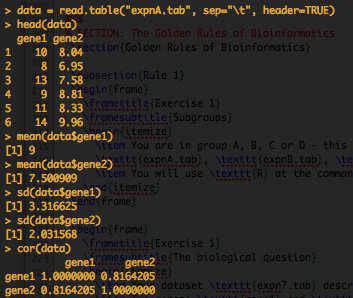
\includegraphics[width=.5\textwidth]{images/ex1_screenshot_b}
\end{frame}

% [fragile] frames must end with \end{frame} directly following a newline, or they break!
  \begin{frame}[fragile]
    \frametitle{Exercise 1}
    \framesubtitle{Load and inspect data in R}
    \begin{lstlisting}[language=R]
> mean(data$gene1)
[1] 9
> mean(data$gene2)
[1] 7.500909
> sd(data$gene1)
[1] 3.316625
> sd(data$gene2)
[1] 2.031568
> cor(data)
          gene1     gene2
gene1 1.0000000 0.8164205
gene2 0.8164205 1.0000000
    \end{lstlisting}
    %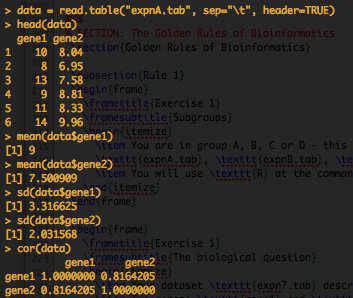
\includegraphics[width=.5\textwidth]{images/ex1_screenshot_b}
\end{frame}

  \begin{frame}
    \frametitle{Exercise 1}
    \framesubtitle{Results}
    \begin{center}
	\begin{tabular}{r|l|l|l|l}
	  measure & expnA & expnB & expnC & expnD \\
	  \hline
	  mean(gene1) & 9     &  &  & \\
	  mean(gene2) & 7.5   &  &  & \\
  	  sd(gene1)   & 3.3   &  &  & \\
  	  sd(gene2)   & 2.0   &  &  & \\  
	  cor(data)   & 0.816 &  &  & \\  
	\end{tabular}
    \end{center}
  \end{frame}

  \begin{frame}
    \frametitle{Exercise 1}
    \framesubtitle{Results}
    \begin{center}
	\begin{tabular}{r|l|l|l|l}
	  measure & expnA & expnB & expnC & expnD \\
	  \hline
	  mean(gene1) & 9     & 9     & 9     & 9 \\
	  mean(gene2) & 7.5   & 7.5   & 7.5   & 7.5 \\
  	  sd(gene1)   & 3.3   & 3.3   & 3.3   & 3.3 \\
  	  sd(gene2)   & 2.0   & 2.0   & 2.0   & 2.0 \\  
	  cor(data)   & 0.816 & 0.816 & 0.816 & 0.816 \\  
	\end{tabular}
	\end{center}
	\begin{itemize}
      \item<2-> $r=0.816 (P<0.005)$ in every experiment
      \item<2-> Can we conclude that \texttt{gene1} and \texttt{gene2} are coexpressed in each experiment?
    \end{itemize}
  \end{frame}

% [fragile] frames must end with \end{frame} directly following a newline, or they break!
  \begin{frame}[fragile]
    \frametitle{Exercise 1}
    \framesubtitle{Plot the data in R}
    \begin{lstlisting}[language=R]
> plot(data)
    \end{lstlisting}
      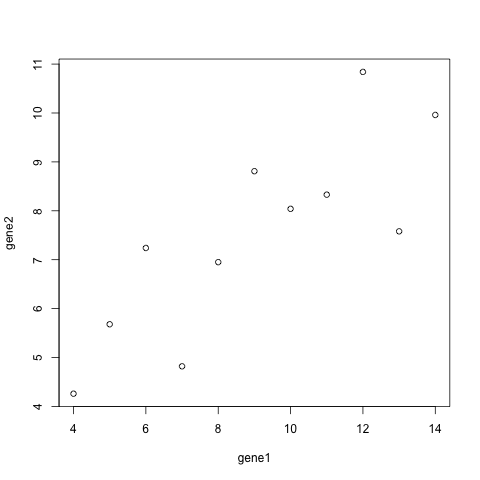
\includegraphics[width=0.4\textwidth]{images/ex1_screenshot_d}        
\end{frame}

  \begin{frame}
    \frametitle{Exercise 1}
    \framesubtitle{Always plot the data}
    Which gene pairs are coexpressed?
    \begin{center}
      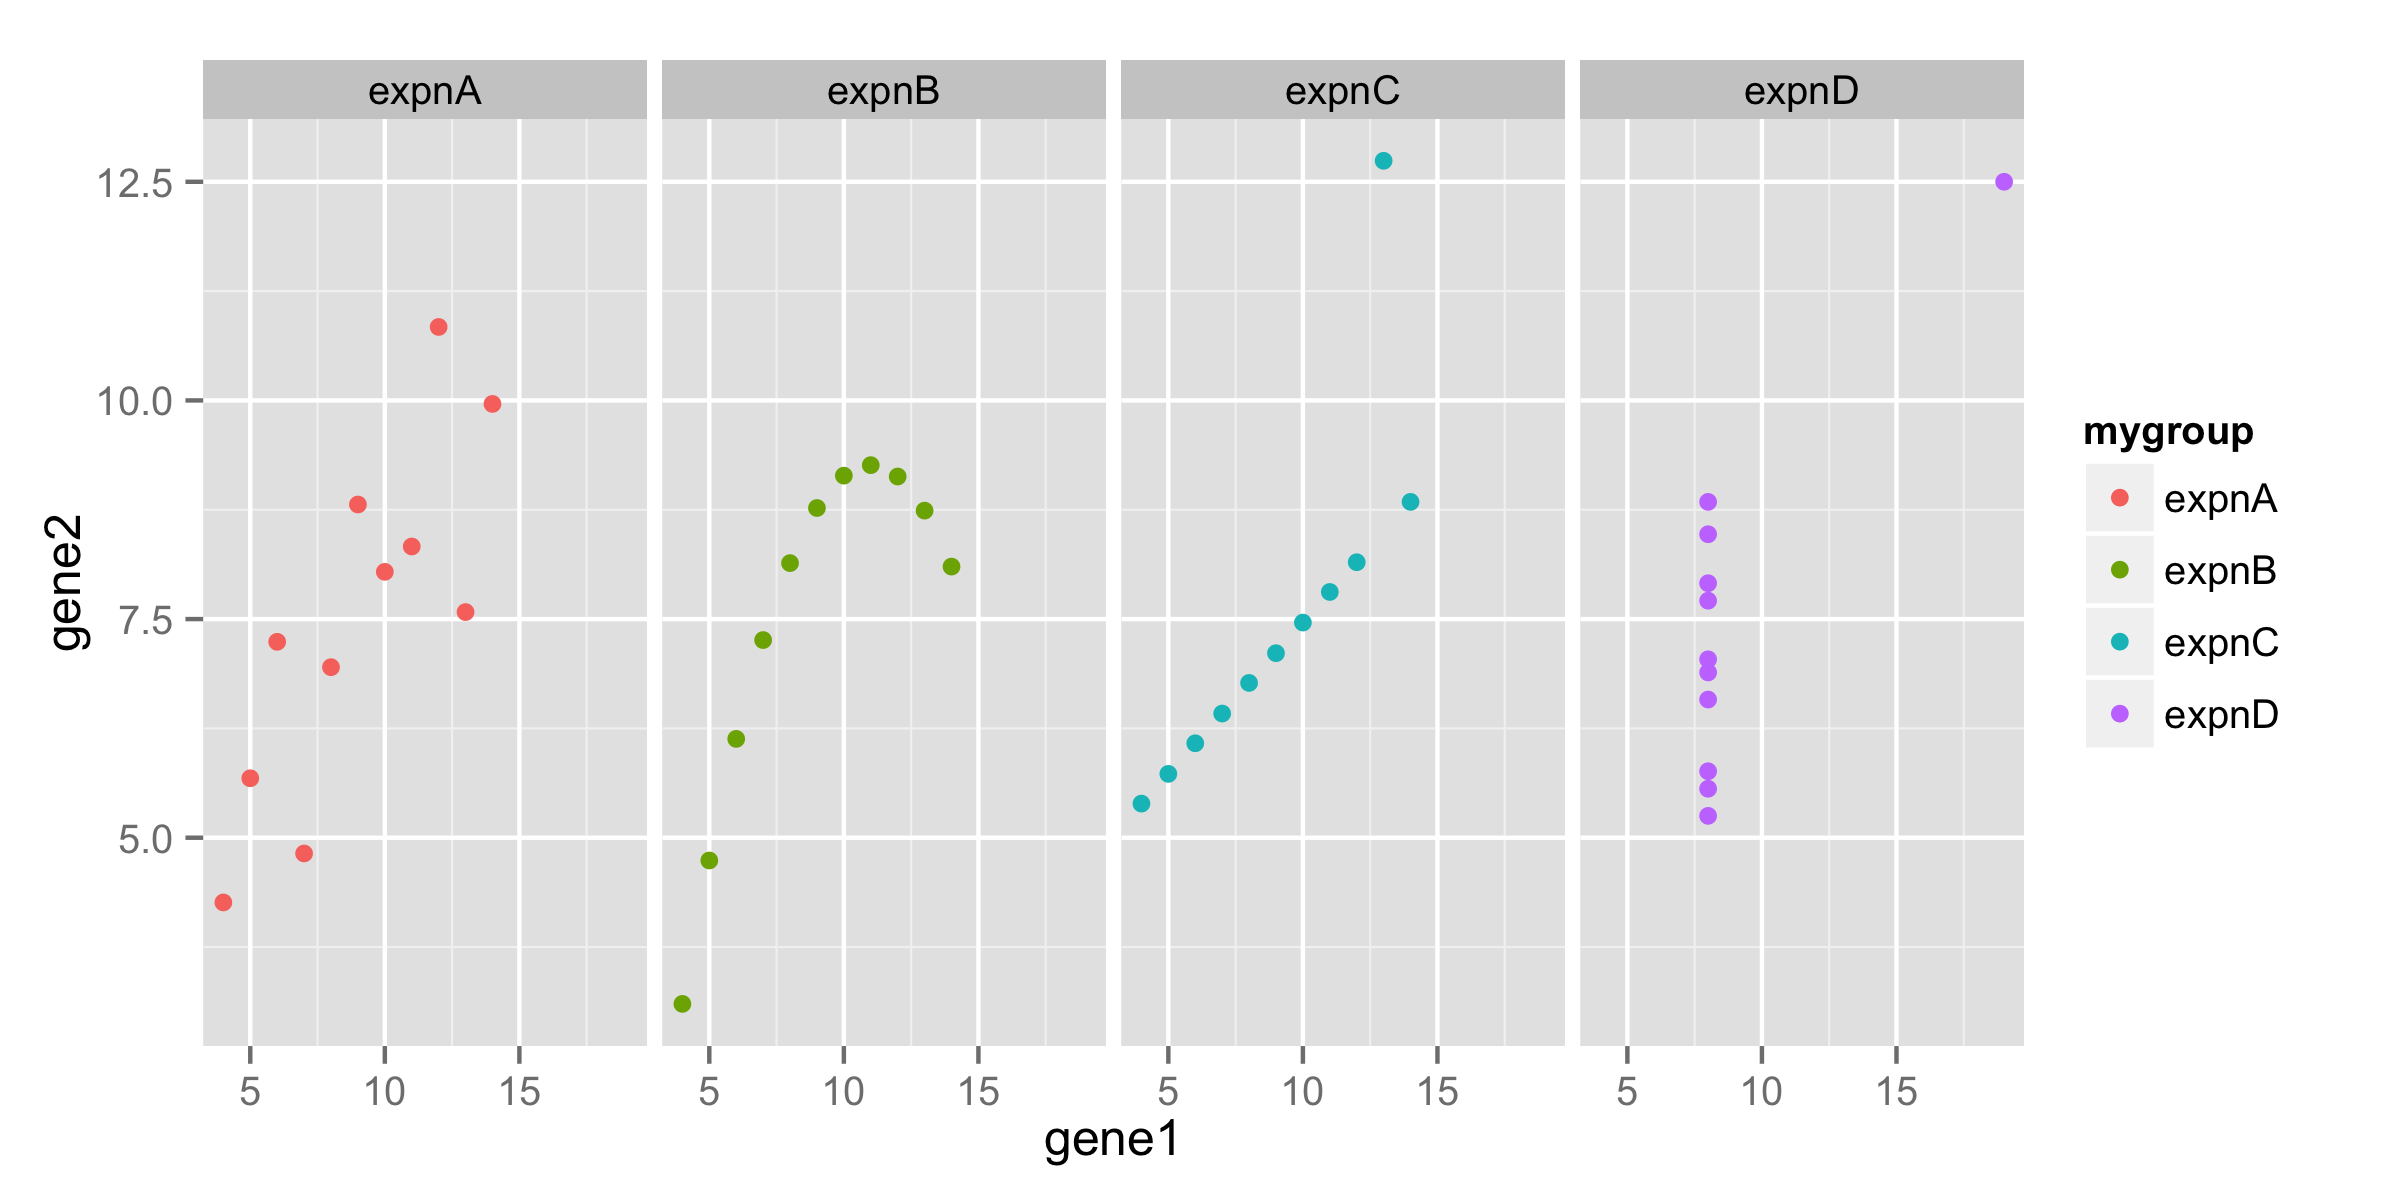
\includegraphics[width=0.9\textwidth]{images/ex1_rplot} \\
    \end{center}
  \end{frame}

  \begin{frame}
    \frametitle{Exercise 1}
    \framesubtitle{Always plot the data}
    Is a matrix of correlation values potentially misleading?
    \begin{center}
      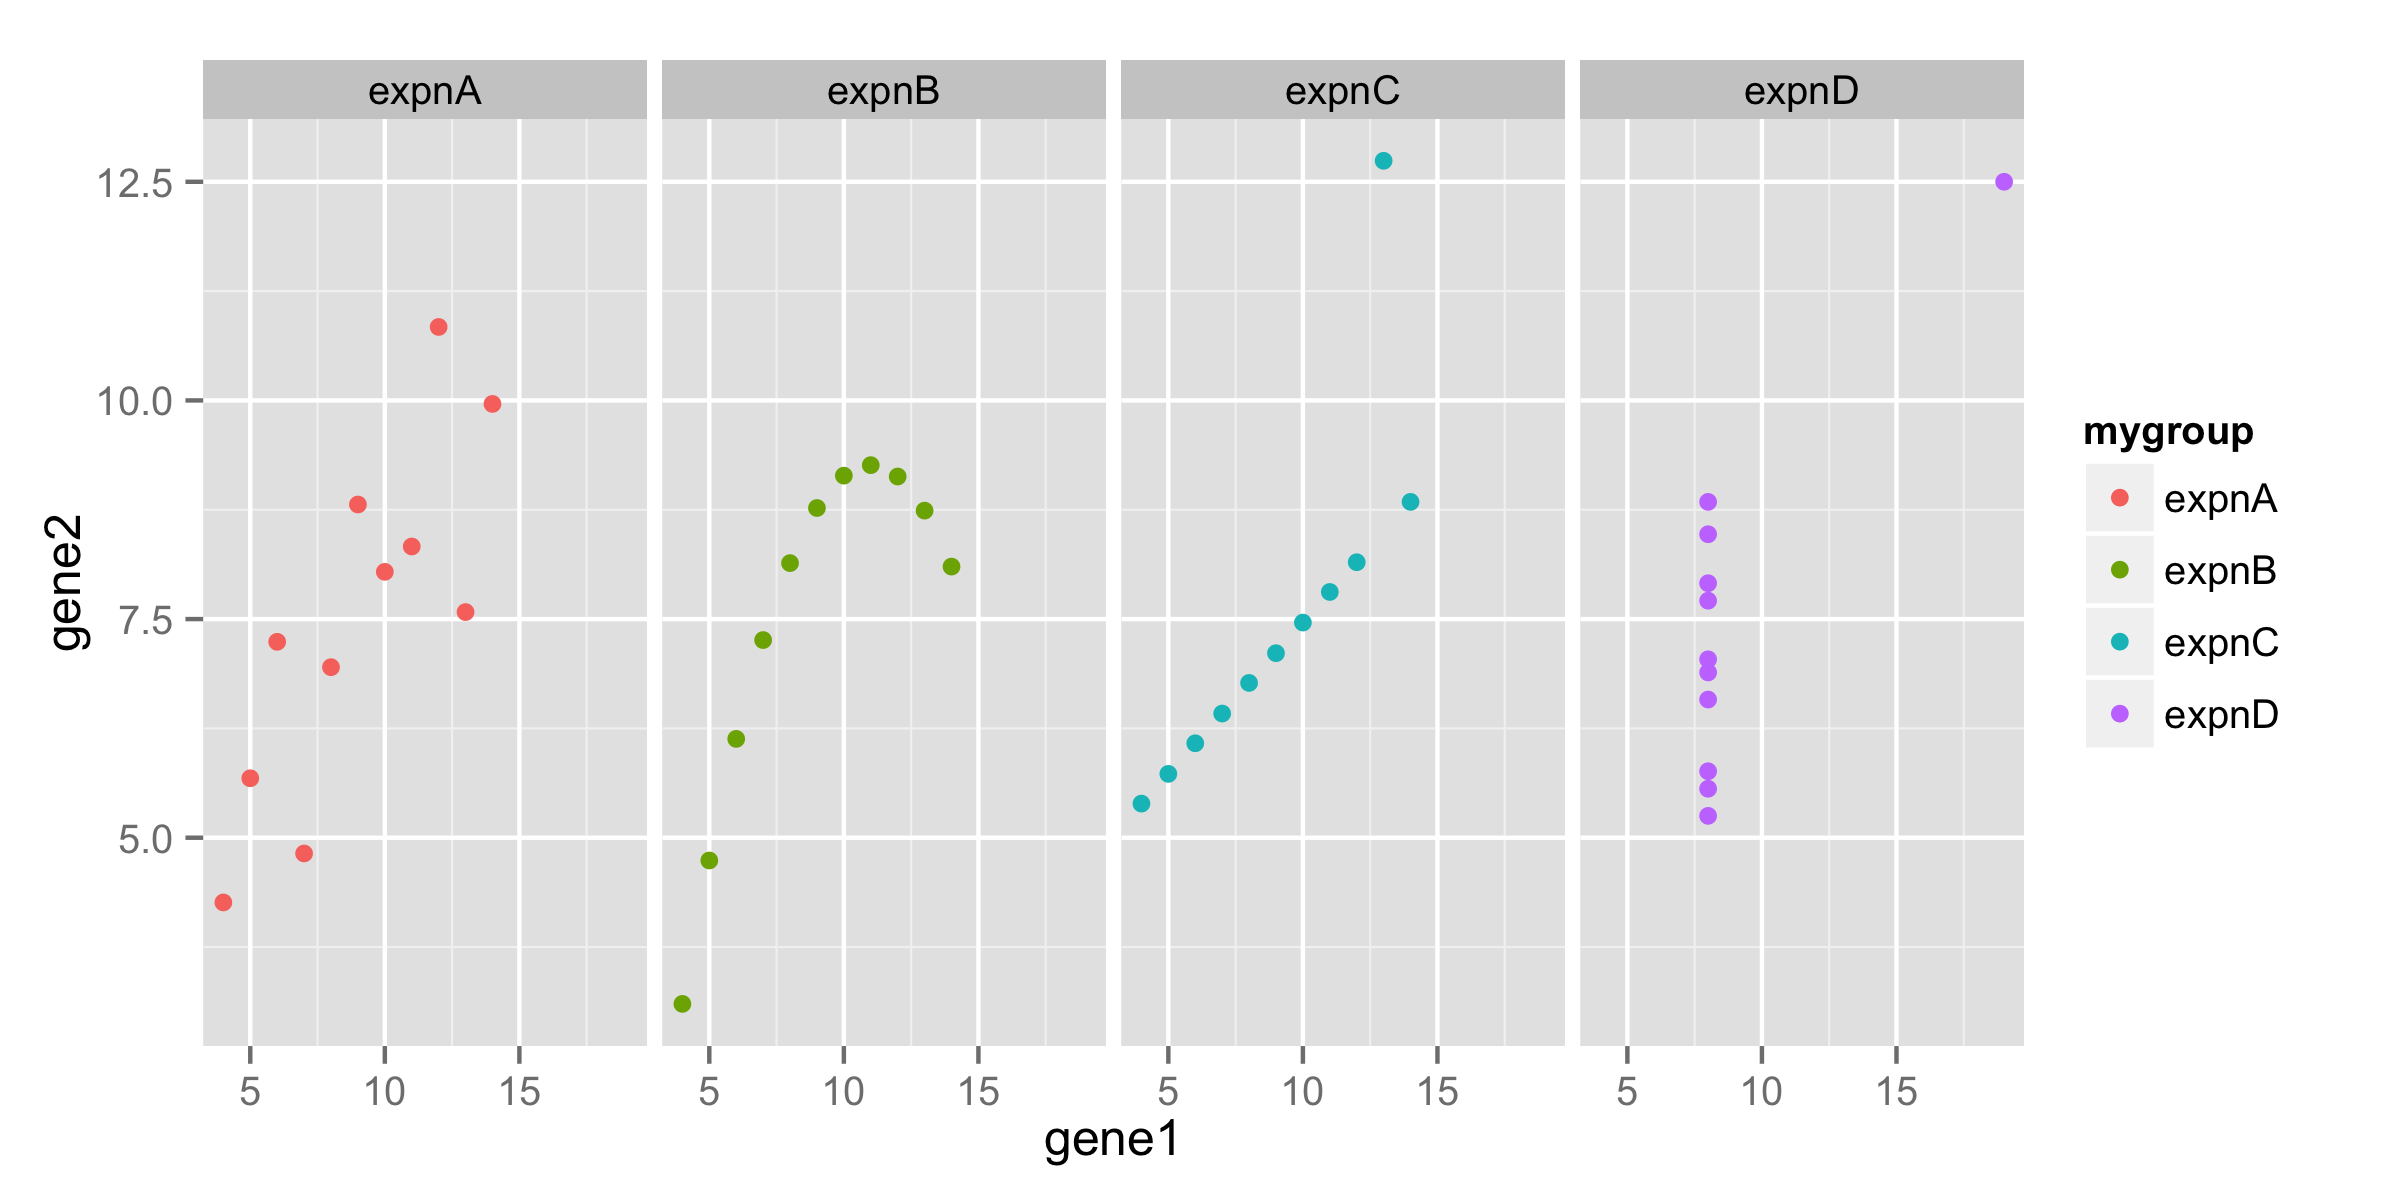
\includegraphics[width=0.9\textwidth]{images/ex1_rplot} \\
    \end{center}
  \end{frame}

  \begin{frame}
    \frametitle{First Golden Rule of Bioinformatics}
    \framesubtitle{Do not trust the data}
	\begin{itemize}
	  \item Always inspect the raw data (trends, outliers, clustering)
	  \item What is the question? Can the data answer it?
	  \item Communicate with data collectors! (don't be afraid of pedantry)
	  \begin{itemize}
	    \item Who? When? How?
	    \item You need to understand the experiment to analyse it (easier if you helped design it).
	    \item Be wary of block effects (experimenter, time, batch, etc.)
	  \end{itemize}
	\end{itemize}
  \end{frame}

  \subsection{Rule 2}
  \begin{frame}
    \frametitle{Exercise 2}
    \framesubtitle{Instructions}    
    \begin{itemize}
      \item You are in group A, B, C or D - this decides your database\\
      \texttt{dbA}, \texttt{dbB}, \texttt{dbC}, \texttt{dbD}
      \item You will use \texttt{BLAST} at the command-line to analyse your data
      \item You will use \texttt{script} at the command-line to record your work
    \end{itemize}
  \end{frame}

% [fragile] frames must end with \end{frame} directly following a newline, or they break!
  \begin{frame}[fragile]
    \frametitle{Exercise 2}
    \framesubtitle{Starting \texttt{script}}    
    \begin{itemize}
      \item Start recording your actions by entering \texttt{script} at the command line      
    \end{itemize}
    \begin{lstlisting}[language=bash]
$ script
Script started, output file is typescript
    \end{lstlisting}    
\end{frame}

% [fragile] frames must end with \end{frame} directly following a newline, or they break!
  \begin{frame}[fragile]
    \frametitle{Exercise 2}
    \framesubtitle{Running \texttt{BLAST}}
    \begin{itemize}
      \item Change directory to the \texttt{ex2\_blast} directory
      \item Run \texttt{BLAST} with the appropriate database
      \item Exit \texttt{script}
    \end{itemize}
    \begin{lstlisting}[language=bash]
$ cd ../ex2_blast
$ blastp -num_alignments 1 -num_descriptions 1 -query query.fasta -db dbA
$ exit
exit
Script done, output file is typescript
    \end{lstlisting}    
\end{frame}

% [fragile] frames must end with \end{frame} directly following a newline, or they break!
  \begin{frame}[fragile]
    \frametitle{Exercise 2}
    \framesubtitle{Viewing \texttt{script} output}
    \begin{itemize}
      \item You can view the \texttt{typescript} file with \texttt{cat}
    \end{itemize}
    \begin{lstlisting}[language=bash]
$ cat typescript
Script started on Fri May  9 10:45:12 2014
lpritc@lpmacpro:$ cd ../ex2_blast
[...]
    \end{lstlisting}    
\end{frame}

% [fragile] frames must end with \end{frame} directly following a newline, or they break!
  \begin{frame}[fragile]
    \frametitle{Exercise 2}
    \framesubtitle{\texttt{BLAST} output}
    \begin{tiny}
    \begin{verbatim}
Query= query protein sequence

Length=400
                                                                      Score
Sequences producing significant alignments:                          (Bits)

  PITG_08491T0 Phytophthora infestans T30-4 choline transporter-l...  34.3


> PITG_08491T0 Phytophthora infestans T30-4 choline transporter-like 
protein (441 aa)
Length=486

 Score = 34.3 bits (77), Method: Compositional matrix adjust.
 Identities = 22/69 (32%), Positives = 38/69 (55%), Gaps = 4/69 (6%)

Query  106  EVILPMMYQFALKPSFADVINDYKPYSKHTAGVSDQELKGEATTWMLADKNSRMKAFLSQ  165
            E+++PM+Y   L   F   ++ Y P   HTA ++  EL+G   T ++A+  S +  F ++
Sbjct  40   ELMVPMLYSLYLVVLFHLPVSAYYP---HTASMTAHELQGAVITILVAETPSIIIQF-AK  95

Query  166  IKTKSNSSE  174
              T SN S+
Sbjct  96   CHTSSNISQ  104
    \end{verbatim}   
    \end{tiny} 
\end{frame}

  \begin{frame}
    \frametitle{Exercise 2}
    \framesubtitle{Results}
    \begin{itemize}
      \item What is a reasonable E-value threshold to call a 'match'?
      \begin{itemize}
        \item 1e-05, 0.001, 0.1, 10?
      \end{itemize}
    \end{itemize}
    \begin{center}
	\begin{tabular}{r|l|l|l|l}
	   & dbA & dbB & dbC & dbD \\
	  \hline
	  \hline
	  E-value &      &  &  & \\
	\end{tabular}
    \end{center}
  \end{frame}

  \begin{frame}
    \frametitle{Exercise 2}
    \framesubtitle{Results}
    \begin{itemize}
      \item What is a reasonable E-value threshold to call a 'match'?
      \begin{itemize}
        \item 1e-05, 0.001, 0.1, 10?
      \end{itemize}
    \end{itemize}
    \begin{center}
	\begin{tabular}{r|l|l|l|l}
	   & dbA & dbB & dbC & dbD \\
	  \hline
	  \hline
	  E-value & 0.45 & 0.002 & 4e-06 & 0.019 \\
	\end{tabular}
    \end{center}
    \begin{itemize}
      \item Five orders of magnitude difference in E-value, depending on database choice - Why?
    \end{itemize}    
  \end{frame}

  \begin{frame}
    \frametitle{Exercise 2}
    \framesubtitle{Results}
    \begin{itemize}
      \item E-values depend on database size
      \item Bit score and alignment do not depend on database size
    \end{itemize}
    \begin{center}
	\begin{tabular}{r|l|l|l|l}
	   & dbA & dbB & dbC & dbD \\
	  \hline
	  \hline
	  E-value & 0.45 & 0.002 & 4e-06 & 0.019 \\
	  Bit score & 34.3 & 34.3 & 34.3 & 34.3 \\
	  \hline
	  Sequences & 100,001 & 501 & 1 & 5,001 \\
	  Letters & 48,650,486 & 210,866 & 486 & 2,066,510 	  
	\end{tabular}
    \end{center}
  \end{frame}

  \begin{frame}
    \frametitle{Exercise 2}
    \framesubtitle{Results}    
    \begin{itemize}
      \item<1-> E-values differ, but the query matches a choline transporter-like 
protein quite well$\ldots$
      \item<2-> \emph{Doesn't it?}
      \item<1-> After all, a biological match is a biological match$\ldots$
      \item<2-> \emph{Isn't it?}
    \end{itemize}
  \end{frame}

% [fragile] frames must end with \end{frame} directly following a newline, or they break!
  \begin{frame}[fragile]
    \frametitle{Exercise 2}
    \framesubtitle{\texttt{BLAST} output}
    \begin{tiny}
    \begin{verbatim}
Query= query protein sequence

Length=400
                                                                      Score     E
Sequences producing significant alignments:                          (Bits)  Value

  PITG_08491T0 Phytophthora infestans T30-4 choline transporter-l...  34.3    4e-06


> PITG_08491T0 Phytophthora infestans T30-4 choline transporter-like 
protein (441 aa)
Length=486

 Score = 34.3 bits (77),  Expect = 4e-06, Method: Compositional matrix adjust.
 Identities = 22/69 (32%), Positives = 38/69 (55%), Gaps = 4/69 (6%)

Query  106  EVILPMMYQFALKPSFADVINDYKPYSKHTAGVSDQELKGEATTWMLADKNSRMKAFLSQ  165
            E+++PM+Y   L   F   ++ Y P   HTA ++  EL+G   T ++A+  S +  F ++
Sbjct  40   ELMVPMLYSLYLVVLFHLPVSAYYP---HTASMTAHELQGAVITILVAETPSIIIQF-AK  95

Query  166  IKTKSNSSE  174
              T SN S+
Sbjct  96   CHTSSNISQ  104
    \end{verbatim}   
    \end{tiny} 
\end{frame}

  \begin{frame}
    \frametitle{Exercise 2}
    \framesubtitle{Remember Golden Rule 1?}    
    \begin{itemize}
      \item<1-> Sequence accessions (\texttt{PITG\_?????T0}) \emph{are} correct in the databases
      \item<2-> Sequence functional descriptions are randomly shuffled: lengths do not match in \texttt{BLAST} output
      \item<3-> \texttt{dbA} contains only three different sequences: two are repeated 50,000 times
      \item<4-> \texttt{query.fasta} is random sequence, not a real protein
      \begin{itemize}
        \item<4-> Shuffled from all \textit{P. infestans} proteins
        \item<4-> No \texttt{nr} or \texttt{PFam} matches        
      \end{itemize}
    \end{itemize}
  \end{frame}

  \begin{frame}
    \frametitle{Second Golden Rule of Bioinformatics}
    \framesubtitle{Do not trust the software}
	\begin{itemize}
	  \item Do not trust the software: it is not an authority
	  \begin{itemize}
	    \item Software does not distinguish meaningful from meaningless data
	    \item Software has bugs
	    \item Algorithms have assumptions, conditions, and applicable domains
	    \item Some problems are inherently hard, or even insoluble
	  \end{itemize}
	  \item You must understand the analysis/algorithm
	  \item Always sanity test
	  \item Test output for robustness to parameter (including data) choice
	\end{itemize}
  \end{frame}

  \subsection{Rule 3}  
  \begin{frame}
    \frametitle{Exercise 3}
    \framesubtitle{Classification}
    \begin{itemize}
      \item Rule: If there is a vowel on one side of the card, there \textit{must} be an even number on the other side.
      \item Which cards \textit{must} be turned over to determine if this rule (if a card shows a vowel on one face, the opposite face is even) holds true?
    \end{itemize}
    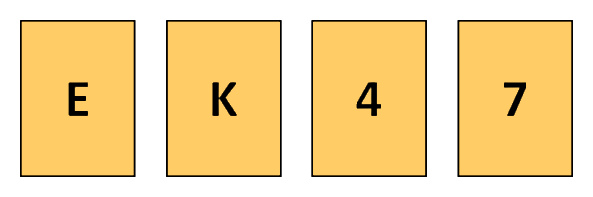
\includegraphics[width=0.8\textwidth]{images/wason}
  \end{frame}

  \begin{frame}
    \frametitle{Exercise 3}
    \framesubtitle{Classification}
    This is the Wason Selection Task
    \begin{itemize}
      \item<1-> If you chose \emph{E} and \emph{4}
      \begin{itemize}
        \item<2-> You are in the typical majority group
        \item<2-> You are not correct
        \item<2-> You have been a victim of confirmation bias (System 1 thinking)
      \end{itemize}
      \item<3-> If you chose \emph{E} and \emph{7}
      \begin{itemize}
        \item<4-> Congratulations!
        \item<4-> Your choice was capable of \textit{falsifying} the rule.
      \end{itemize}
    \end{itemize}
  \end{frame}

  \begin{frame}
    \frametitle{Exercise 3}
    \framesubtitle{Classification}
    Only questions that necessarily \emph{test} the rule should be asked
    \begin{center}
	\begin{tabular}{c|c|c}
	  Card & Outcome & Rule \\
	  \hline
	  \hline
	    \multirow{2}{*}{E} & Even & Can be true even if rule false \\
	                                & Odd & \emph{violated} \\
	  \hline
	    \multirow{2}{*}{K} & Even & na \\
	                                & Odd & na \\	    
	  \hline
	    \multirow{2}{*}{4} & Vowel & Can be true even if rule false \\
	                                & Consonant & na \\
	  \hline
	    \multirow{2}{*}{7} & Vowel & \emph{violated} \\
	                                & Consonant & na \\	    
	\end{tabular}
    \end{center}
  \end{frame}

  \begin{frame}
    \frametitle{Exercise 3}
    \framesubtitle{Classification}
    \begin{itemize}
      \item This is equivalent to protein functional classification
      \item Rule: If there is a CRN/RxLR/T3SS domain, the protein \textit{must} be an effector.
    \end{itemize}
    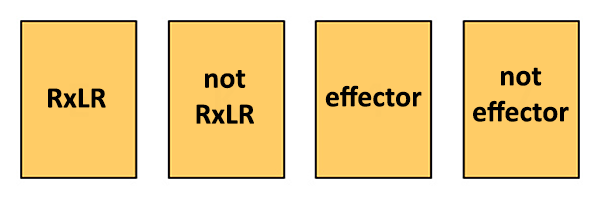
\includegraphics[width=\textwidth]{images/wason_rxlr}
  \end{frame}
  
  \begin{frame}
    \frametitle{Exercise 3}
    \framesubtitle{Classification}
    \begin{itemize}
      \item Wason Selection Task
      \begin{itemize}
        \item An uninformative experiment is performed
        \item \url{http://en.wikipedia.org/wiki/Wason_selection_task}
      \end{itemize}
      \item Affirming the Consequent (a related formal fallacy)
      \begin{enumerate}
       \item If $P$, then $Q$
       \item $Q$
       \item Therefore, $P$
      \end{enumerate}
      \begin{itemize}
        \item Experimental results are misinterpreted
        \item \url{http://en.wikipedia.org/wiki/Affirming_the_consequent}
      \end{itemize}
    \end{itemize}
  \end{frame}

  \begin{frame}
    \frametitle{Third Golden Rule of Bioinformatics}
    \framesubtitle{Don't trust yourself}
	\begin{itemize}
	  \item Everyone has expectations of their data/experiment
	    \begin{itemize}
	      \item Beware cognitive errors, such as confirmation bias!
	      \item System 1 vs. System 2 $\approx$ intuition vs. reason
	    \end{itemize}
	  \item Think statistically! 
	    \begin{itemize}
	      \item Large datasets can be counterintuitive.
	      \item Always account for multiple tests.
	    \end{itemize}
	  \item Use test-driven development of analyses and code
	    \begin{itemize}
	      \item Use examples that pass \textit{and} fail
	    \end{itemize}	  
	\end{itemize}
  \end{frame}

  \begin{frame}
    \frametitle{Conclusions}
	\begin{itemize}
	  \item \emph{Always communicate!}
	    \begin{itemize}
	      \item worst errors are silent
	    \end{itemize}	  
	  \item Don't trust the data
	    \begin{itemize}
	      \item formatting/validation/category errors
	      \item suitability for scientific question
	    \end{itemize}
	  \item Don't trust the software
	    \begin{itemize}
	      \item software is not an authority
	      \item always benchmark, always validate
	    \end{itemize}
	  \item Don't trust yourself
	    \begin{itemize}
	      \item beware cognitive errors
	      \item think statistically
	      \item biological "stories" can be constructed from nonsense
	    \end{itemize}	  
	\end{itemize}
  \end{frame}

%%%% SPARES
%% SECTION: 
%  \section{}
%
%  \begin{frame}
%    \frametitle{Third Golden Rule of Bioinformatics}
%    \framesubtitle{Keep raw data and analysis separate}
%	\begin{itemize}
%	  \item Keep raw data and analysis separate
%	  \item Avoid Excel! (off-by-one/copy errors/risk of changing data)
%	  \item Make raw data read-only, and back it up immediately
%	\end{itemize}
%  \end{frame}
%
%
%  \begin{frame}
%    \frametitle{Programming}
%   % \framesubtitle{Keep raw data and analysis separate}
%	\begin{itemize}
%	  \item Programming is like writing a book$\ldots$
%	  \item $\ldots$except that if you miss out a comma on p.126, the whole thing makes no damned sense!
%	\end{itemize}
%  \end{frame}
%
%  \begin{frame}
%    \frametitle{Assessing Performance}
%    \framesubtitle{Contingency Tables}
%    \begin{center}
%	\begin{tabular}{cc|c|c|}
%	  \cline{3-4}
%		& & \multicolumn{2}{|c|}{Condition (Gold standard)}\\
%	  \cline{3-4}
%		& & True & False \\
%	  \hline
%	  \multicolumn{1}{ |c| }{\multirow{2}{*}{Test outcome}}& 
%	  \multicolumn{1}{ |c| }{Positive} & True Positive \cellcolor{green} & 
%	    False Positive\cellcolor{red}\\
%	  \cline{2-4}
%	  \multicolumn{1}{ |c| }{} & \multicolumn{1}{ |c| }{Negative} & 
%	    False Negative\cellcolor{red} & True Negative \cellcolor{green}\\
%	  \hline
%	\end{tabular}
%	\end{center}
%  \end{frame}
%
%  \begin{frame}
%  \end{frame}

% etc
\end{document}